\subsection{CIVIS Platform Design Concept}
\label{sect:design_concept}

Considering the analytical frames and the CIVIS use cases, we chose a set of CIVIS platform features and translated those into three self-contained and composable parts to be included in the CIVIS (front-end) application (hereinafter abbreviated as CIVIS app)\footnote{A shortened list of YouPower app mock-ups can be found at \url{http://civis.tbm.tudelft.nl/mockups/}.}: 
\begin{enumerate}
\item \nameref{sect:tips}
\item \nameref{sect:brf}
\item \nameref{sect:load_shifting}
\end{enumerate}



With peer review results and users' feedback on the design, adaptations and changes are made to suit user needs and to achieve the CIVIS research goal. 
In general, the application aims to enhance users' energy know-how through action suggestions that are implementable in everyday life, engage users in energy communities with understandable and actionable information and feedback, and facilitate community interaction and self-teaching by means of group discussions.
%

Given the time and resource constraints, the app can not be developed all-in-one cross-platform (for phones, tablets and computers). We chose to design the front-end as a mobile app. This means that the app design has layouts and user interactions that suit (small) phone screens. %The consideration is multi-fold. 
Western Europe has a large mobile phone internet user base\footnote{
Between 2013 and 2017, the penetration rate of mobile phone internet users among mobile phone users will rise from 49.0\% to 77.8\%. See more at:\url{ http://www.emarketer.com/Article/Nearly-Half-of-Western-Europeans-Will-Use-Mobile-Web-This-Year/1010510\#sthash.AaVfsqIU.dpuf}}. Many surveys show that mobile apps have advantages such as creating deeper user engagement, easy sharing, among others\footnote{\url{https://infomedia.com/blog/the-advantages-of-mobile-apps/}, \url{https://econsultancy.com/blog/62326-85-of-consumers-favour-apps-over-mobile-websites/}}. This makes mobile app a good choice given the goal of the CIVIS platform. Once developed, mobile apps can also be more easily transformed to web browser versions, while the reverse is more difficult. The back-end of the CIVIS platform will remain mostly the same independent of the front-end alternatives. 


\subsubsection{Action Suggestions (Both Test Sites)}
\label{sect:tips}

\paragraph{Design Concept}

The ``action suggestions'' part of the app can be used in both test sites. 
It aims to provide users easy access to practical and inexpensive action suggestions to (1) inform users' energy know-how, (2) stimulate users' awareness, and to (3) shape users' long-term behavior related to household energy consumption. Users can follow a few actions at a time and are suggested with a new action when one is completed. A user is prompted with suggestions such as: 
\begin{itemize}
	\item Defrost your freezer regularly, e.g., every two months or when ice starts to form. 
	\item If possible, shower rather than bath, as a short shower will use less hot water. Shower quickly. 
	\item When cooking on top of your range, match the size of the pan to the heating element.
	\item Find and seal up leaks. Do you have leaks at home? Look for places where you have pipes, vents or electrical conduits ... 
\end{itemize}

Each action is accompanied with a short explanation and the information about how many people are already taking this action, and the estimated impact and effort (on a scale of 1 to 5) of performing the action so that the user knows what to expect. The user is asked whether s/he wants to follow an action; see Figure~\ref{fig:action_choice} for an example. 
%
% 
Some suggestions can be triggered by time, e.g., ``Defrost your fridge in $x$ days.'' ($x$ to be set by users themselves.) In such cases, the app reminds the users of the (pending) actions they are interested in. 
A user has an ``action list'' that registers the user's actions. 

\begin{figure}
\begin{center}
	   	 \frame{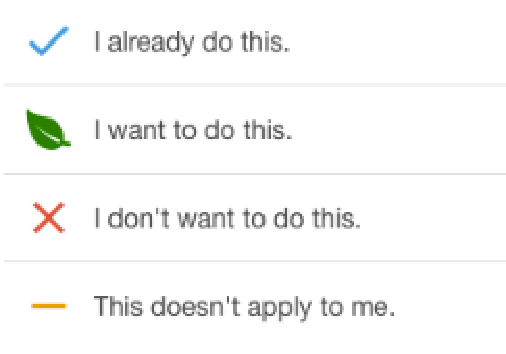
\includegraphics[width=.4\textwidth]{img/action_choice.pdf}}\caption{A user's choices to accept or reject an action suggestion}\label{fig:action_choice}
\end{center}
\end{figure} 

\begin{figure}
\begin{center}
	   \frame{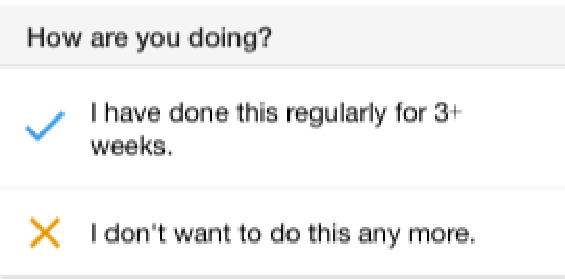
\includegraphics[width=.44\textwidth]{img/action_how.pdf}}\caption{A user's choices to complete or abandon an accepted action}\label{fig:action_how}
\end{center}
\end{figure} 

When a user completes an action, the user is awarded with points (displayed as \textit{Leaves}) associated to the effort and impact level of that action. 
A user may also choose to abandon an accepted action. See Figure~\ref{fig:action_how}. In both cases, the user is asked to give feedback; Figures~\ref{fig:action_completed} and \ref{fig:action_not_completed}. 
A user may ``like'' or ``share'' an action, rate the effort level of performing this action, reflect on her/his performance, give comments to the action, ``like'' the others' comments, and let us know what went wrong. 

\begin{figure}
\begin{center}
	\begin{minipage}[t]{0.44\textwidth}
	   \frame{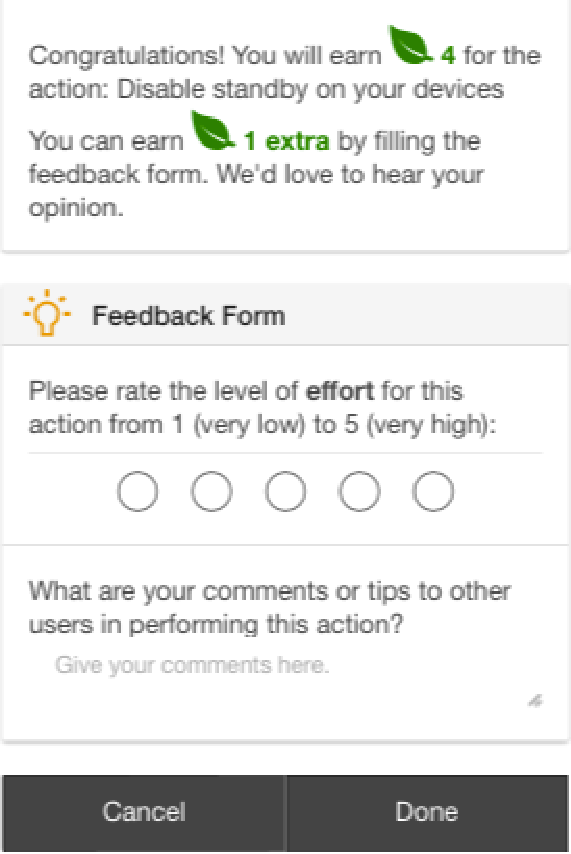
\includegraphics[width=\textwidth]{img/action_completed.pdf}}
	    \caption{The feedback form when a user completes an action.}\label{fig:action_completed}
	  \end{minipage}
	  \hfill
	\begin{minipage}[t]{0.44\textwidth}
	   \frame{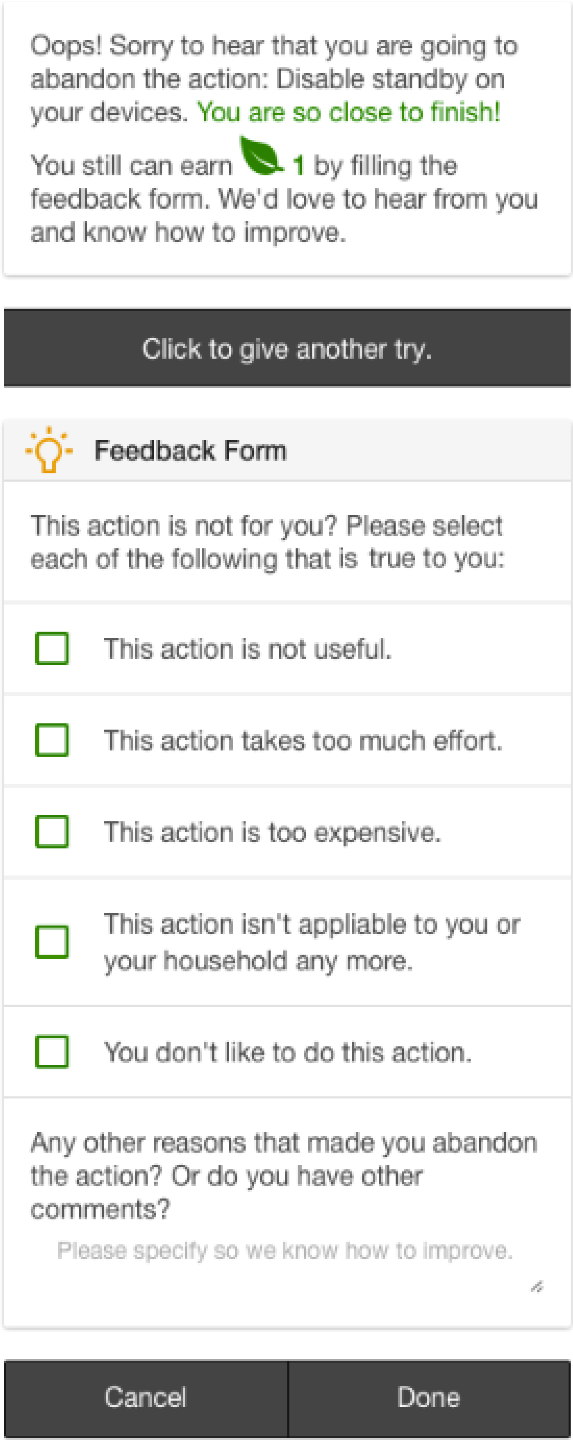
\includegraphics[width=\textwidth]{img/action_not_completed.pdf}}
	   \caption{The feedback form when a user abandons an action.}\label{fig:action_not_completed}
	  \end{minipage}
\end{center}
\end{figure} 

We chose to use leaves for the counting to promote intrinsic pro-environmental values. With the current design, users can collect leaves when they completed an action or when they give comments or feedbacks on the CIVIS application. The details of how the leaves can be collected (in an engaging way) will be adapted to user feedback or improved based on the actual result after deployment at the test sites. 

\paragraph{Be Engaged in Household and Communities}

To engage each member in a household, the app allows a user to add members (who are also the CIVIS app users) to his/her household. The family/household is the original cell of social life. Being involved in and contributing to household responsibilities is the first step of taking responsibilities towards communities and the society in general. 
A user can see the actions of household members, add the actions to his/her own list, and reflect on their collective actions.
% 
A user can also join a community. The top actions (the ones with most participants) in a community are displayed to members to introduce social norms. 
A user can also participate in community discussions to exchange ideas and share their experiences. 


%This application allows users to create and participate in community and personal energy challenges. It gives participants feedback on their performance during the challenge period and provides encouragement for participation using micro-actions. Users who performed well can share their success stories with other users. The application also allows for friends and group discussion. The community challenges can be incentivised by local investments (solar panels for the building), or through funding projects in developing countries (a school in Uganda). This application tries to motivate user engagement in energy community.

\paragraph{About the Actions}
Currently, we composed a list of about 50 actions\footnote{\url{https://goo.gl/R11QdZ}} to be suggested to the users. These actions are from credible sources such as different national and international energy agencies or associations. Many actions we selected are practical and inexpensive to implement in everyday life. These include routine actions such as ``don't keep hot water flowing when you wash your dishes by hand'', regular actions such as ``defrost your fridge in $x$ days'' and one time actions such as ``installing a programmable thermostat''.  The explanation of the actions mainly focuses on intrinsic values to target long-term sustainable behaviors. 

\paragraph{Feedback on Achievements}
In order to keep users motivated, we implement a set of achievements that are unlocked over time by using the app and performing the actions. For instance, users can get an achievement notification after they have performed a certain number of actions, accumulated a certain number of leaves individually or as part of some community, or after they have been using the app regularly for a certain period of time. Whenever a user unlocks an achievement in some category, s/he gets informed what is the next achievement in this category that s/he can reach. (E.g. ``Congrats! You completed your first $3$ actions! Your next goal is $5$ actions. Keep it up!'') Such achievements are based on the goal-setting \citep{Abrahamse2007265} and individual and collective feedback \citep{Abrahamse2013} approaches to behavioral changes in energy consumption.

\paragraph{Personalization and Localization}
A user can set a personal profile and a household profile. We allow a user to customize his/her display name, nickname, preferred language (English, Italian or Swedish), photo, etc., and to provide information about his/her household composition, home type/size, important electrical appliance items, etc. The information is useful for giving personalized suggestions, the comparison of similar households and/or individuals, and can be used by us for research purposes. When a user wants to link the app to the household's (sensors and/or DSO) energy data, the household's data account has to be provided. 
% 
The app customizes its content to a user's test site: housing cooperative for the Swedish site and load-shifting for the Italian site. They will be discussed in the next two subsections. 




\paragraph{Design Evaluation}
The design was evaluated by peer reviews, a study with 24 participants in an environmentally-oriented event in Helsinki\footnote{\url{https://oscedays.org/helsinki/}}, and a workshop with 9 participants in the Italian test site. 
In general, people liked the idea of receiving suggestions (tips) about what to do. 
They would like to see the impact of their actions and asked for easy to perform actions. The majority of the users were interested in cooperative/community actions, e.g., to save together and to donate for a common goal; very few showed interest in competition. 
Some suggested that for those who are not comfortable with smart-phones (or have none), the app should be made available through a browser. 

% 
Some people mentioned that the connection (or difference) between the \textit{Suggestions} and the \textit{Challenges} is hard to understand. Challenges were designed to express personal or community energy-goals, while suggestions are the means to achieve the goals. We later changed the name of this feature from \textit{Challenges} to \textit{Achievements}. 

Some people asked for the authority of the suggestions: it isn't clear where the tips come from. To what extent can they be trusted? Are they results of applied research? This is not marginal in a community of people who are quite familiar with energy-related issues. Having an explanation of how trustworthy these tips are would be very important. 
%
The meaning and value of the leaves are also another aspect that was questioned the most. 
We thus decided to have an information page so that a number of such issues can be explained to the users. 
In addition, users can send feedback to CIVIS through the app to keep the designers updated of users' concerns, questions, or other issues. 

Some participants think that other people (in their neighborhood or city) do not put the same effort in energy conservation as themselves. The CIVIS approach to display other's energy actions in the app may have the potential to motivate people seeing others' efforts.

Many expressed the opinion that monetary savings are only somewhat important to them, and they were also skeptical about how much money they can actually save. The participants show interest to learn about energy saving strategies, as they are driven by more intrinsic motives.




